\section{Hiérarchie arithmétique}


Dans cette sections nous allons étudier les formules arithmétiques du premier ordre sous forme prenexe et comment les classifier.



\begin{definition}[Formules arithmétiques du premier ordre]
	Les formules arithmétiques du premier ordre sous forme prenexe sont construites selon la grammaire suivante :

	\begin{syntaxdef}
		\syntaxHeader {v} {x,y,z,x_1,y_1,z_1,\ldots} {Variables}
	\end{syntaxdef}

	\begin{syntaxdef}
		\syntaxHeader {e} {v} {Variable}
		\syntax {0,1,2,3,4,\ldots} {Nombre dans $\N$}
		\syntax {e + e} {Addition}
		\syntax {e * e} {Multiplication}
		\syntax {S(e)} {Fonction successeur}
	\end{syntaxdef}

	\begin{syntaxdef}
		\syntaxHeader {\phi} {e \leq e} {Variables}
		\syntax {\phi \land \phi} {Conjonction}
		\syntax {\phi \lor \phi} {Disjonction}
		\syntax {\lnot \phi} {Négation}
		\syntax {(\phi)} {Expressions parenthésées}
	\end{syntaxdef}

	\begin{syntaxdef}
		\syntaxHeader {\psi} {\phi} {Formule sans quantificateur}
		\syntax {\exists x \psi} {Quantificateur existentiel}
		\syntax {\forall x \psi} {Quantificateur universel}
	\end{syntaxdef}


	Une formule est prenexe si tous ses quantificateurs "à gauche".
	$(\forall x (x \leq 2)) \land  (\forall y (2 \leq y))$ n'est pas sous forme prenexe mais
	$(\forall x \forall y ((x \leq 2) \land  (2 \leq x))$ l'est.

	Ainsi, toute formule $\psi$ est prenexe par construction.
\end{definition}



\begin{definition}

	On défini les ensembles :

	\begin{eqnarray*}
		\Sigma_{n + 1} &=& \setdef { \exists x \psi } {\psi \in \Pi_n}  \\
		\Pi_{n + 1} &=& \setdef { \forall x \psi } {\psi \in \Sigma_n}  \\
		\Delta_{n + 1} &=& \Sigma_{n + 1} \cap \Pi_{n + 1} \\
		\Delta_0 &=& \Pi_0 = \Sigma_0= \phi \reason {$\phi$ sans quantificateurs non bornés}
	\end{eqnarray*}

	Autrement dit, $\Sigma_n$ est l'ensemble de formules avec $n$ quantificateurs alternés qui commence par un quantificateur existentiel.
\end{definition}

\begin{prop}
	$\Delta_0$ est un ensemble calculable.
\end{prop}

\begin{proof}
	Soit $\phi \in \Delta_0$, alors, comme elle ne contient pas de quantificateurs non bornés, alors on peut essayer toutes les valeurs possibles, car il y a un nombre
	fini.
\end{proof}


Dans cette section nous allons étudier les relations entres ce ensembles afin de pouvoir les classifier, aboutissant a la hiérarchie de la Figure \ref{fig:arith-hier}.


\begin{figure}[h]
	\begin{center}
		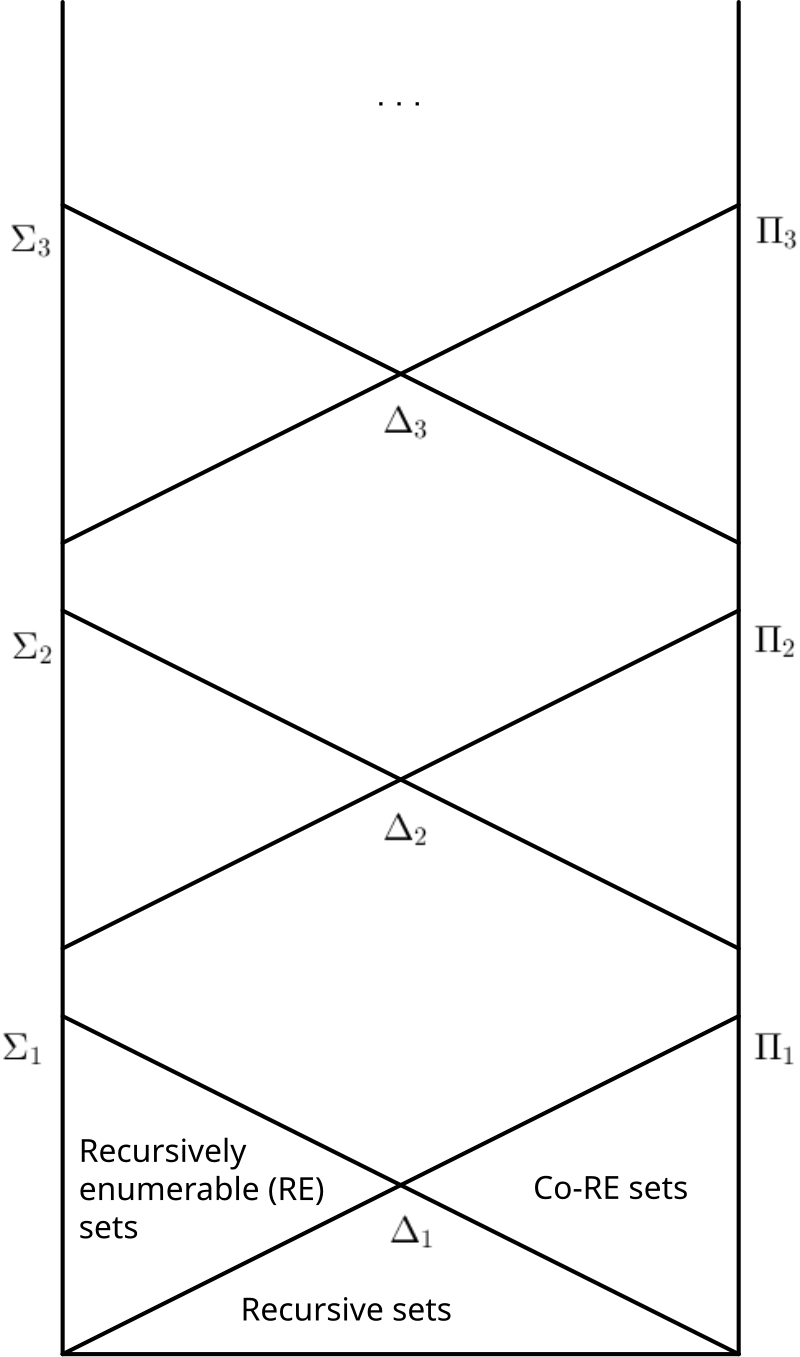
\includegraphics[height=7cm]{./images/Arithmetic_hierarchy.png}
	\end{center}
	\caption{Hiérarchie arithmétique}
	\label{fig:arith-hier}
\end{figure}



\begin{definition}[eval]
	On note $eval(\encode M, w, n)$ la machine que simule l'exécution de $M$ sur $w$ en au plus $n$ étapes.
\end{definition}

\begin{prop}[Admis]
	$eval$ est décidable.
\end{prop}


\begin{exercice}
	Montrer que $ACCEPT = \setdef {\encode {M,w}} {M(w) = 1} \in \Sigma_1$
\end{exercice}

\begin{proof}
	$$\phi (M,w) =  \exists n, \ \underbrace{eval(\encode M, w, n) = 1}_{\in \Delta_0} \in \Sigma_1$$

	Ainsi, $\phi$ décrit $ACCEPT$ et $\phi \in \Sigma_1$ et donc $ACCPET \in \Sigma_1$.
\end{proof}


\begin{exercice}
	Montrer que $ACCEPT$ est $\Sigma_1$-complet, \ie
	$$ \forall L \in \Sigma_1, L \leqm ACCEPT $$
\end{exercice}

\begin{proof}

	Soit $L \in \Sigma_1$. Alors il existe $\phi \in \Delta_0$ \tq
	$$ L = \setdef {n} {\exists x \phi(x,n)} $$

	Soit $M(n)$ la machine qui énumere tous les $x$ et accepte si $\phi(x,n)$ est satisfaite.
	Alors $M$ reconnait $L$.
\end{proof}


\iffalse
	\begin{prop}
		$L$ est r.e. $\implies L \in \Sigma_1$.
	\end{prop}

	\begin{proof}
		\begin{eqnarray*}
			L \text{ est r.e.} &\iff& (\forall w, w \in L \iff \exists x, eval (\encode M,w,x) = 1)\\
			&\implies& L \in \Sigma_1
		\end{eqnarray*}
	\end{proof}
\fi


\begin{prop}
	$RE = \Sigma_1$
\end{prop}

\begin{proof}
	$$L \text{ est r.e.} \iff \exists L_d \text{ décidable }, L = \setdef {w} {\underbrace{\exists w', \encode {w, w'} \in L_d}_{\phi}}$$
	Et donc $RE = \Sigma_1$
\end{proof}

\subsection{Machines à oracle}

\begin{definition}[Machine de Turing à oracle]
	Une Machine à oracle est une machine de Turing qui a access a une fonction $\fmots {\mathscr O}$ pendant son execution: elle a donc, en plus de la machine
	initiale, un ruban d'appel (pour l'oracle) et un état special d'appel.

	Si la machine de rentre dans l'état d'appel avec $u \in \mots$ sur le ruban, alors $\mathscr O (u) \in \mots$ est écrit sur le ruban d'appel.
\end{definition}

\begin{definition}[Reconnaissance]

	On dit que $M$ reconnait $L$ relativement a un oracle $A$ si
	$$ \forall w, M^A (w) = 1 \iff w \in L $$
	où $M^A$ est l'exécution de $M$ avec l'oracle $A$.

\end{definition}

\begin{definition}[Reduction de Turing]
	On dit que $A \leqt B \iff A$ est décidable relativement à $B$.
\end{definition}

\begin{remarque}
	On a que $A \leqm B \implies A \leqt B$ (il suffit de prendre la fonction de reduction $f$ comme l'oracle).
\end{remarque}

\begin{remarque}
	Pour tout langage $L$ on a que $L \leqt \bar L \et \bar L \leqt L$ et dont $L \equivt \bar L$.
\end{remarque}


\subsection{Hiérarchie arithmétique}

\begin{lemma}
	Si $A$ est $C$-complet:  $\exists Y$ tel que $X$ est $re(Y)$ avec $Y \in C$ $\iff$ $X$ est $re(A)$.
\end{lemma}

\begin{theorem} [de post]
	Nous avons les résultats suivants :
	\begin{enumerate}
		\item
		      \begin{enumerate}
			      \item
			            \begin{eqnarray*}
				            L \in \Sigma_{n+1} &\iff& L \text{ est r.e. relativement  un langage }  \Pi_n  \\
				            &\iff& L \text{ est r.e. relativement  un langage }  \Sigma_{n}
			            \end{eqnarray*}

			      \item
			            \begin{eqnarray*}
				            L \in \Pi_{n+1} &\iff& L \text{ est co-r.e. relativement  un langage }  \Sigma_n  \\
				            &\iff& L \text{ est r.e. relativement  un langage }  \Pi_n
			            \end{eqnarray*}
		      \end{enumerate}

		\item Il existe un langage $\Sigma_n$ complet, noté $\emptyset^{(n)}$.
	\end{enumerate}
\end{theorem}


\begin{definition}[Saut de Turing]
	Soit $X$ un langage,

	$X' = \setdef c {\phi_c^X(c) \text{ est défini}} = \setdef {\encode M} {M^X \text{ s'arrete sur } \encode M}$

	$\phi_{c \in \mots}$ : énumeration des fonctions calculables.

	$\phi_{c \in \mots}^X$ : énumeration des fonctions calculables relativement à $X$. Et donc $\phi_{\encode M}^X(w) = M^X(w)$
\end{definition}


\begin{exemple}
	$$\emptyset' = \setdef {\encode M} {M^{\emptyset} \text{ s'arrete sur } \encode M} \equivm \halt$$
\end{exemple}

\begin{exercice}
	Montrer que $\emptyset '$ est $\Sigma_1$-complet :
	\begin{enumerate}
		\item $\emptyset' \in \Sigma_1$
		\item $\forall L \in \Sigma_1, L \leqm \emptyset'$
	\end{enumerate}
\end{exercice}

TODO
